\chapter{Contador Ascendente}
El circuito electr\'onico de un contador est\'a compuesto por flip flops tipo T ya que estos pueden almacenar un bit el cual se lo llama estado y proporcionan la facilidad de invertir el estado cuando ocurre el evento del flanco ascendente del clock. Es decir, se produce un toggle.
\section{Funcionamiento Lógico del Contador Ascendente}
El funcionamiento lógico del contador se lo explica en la siguiente tabla:
\begin{center}
	\begin{table}[h!]
		\begin{center}
			\caption{Tabla de Verdad del Contador (3 bits)}
			\begin{tabular}{|c|c|}
				\hline
				%\textbf{INPUT} & \textbf{OUTPUT} \\
				%\hline
				\textbf{Clock Cycle} & \textbf{Q2 Q1 Q0} \\
				\hline
				0 & 0 0 0\\
				\hline
				1 & 0 0 1\\
				\hline
				2 & 0 1 0\\
				\hline
				3 & 0 1 1\\
				\hline
				4 & 1 0 0\\
				\hline
				5 & 1 0 1\\
				\hline
				6 & 1 1 0\\
				\hline
				7 & 1 1 1\\
				\hline
				0 & 0 0 0\\
				\hline
			\end{tabular} \\
		\end{center}
	\end{table}
\end{center}
Donde el clock cycle simboliza el número de flancos ascendentes que se van presentando. Y siendo Q2, Q1 y Q0 los estados que cada flip flop almacena.

\section{Tipos de Contadores}
Los dos tipos básicos de contadores son el sincrónico y al asincrónico. A continuación se muestran los circutios electrónicos de cada uno.

\begin{center}
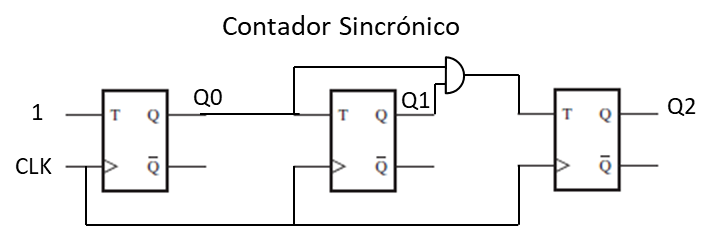
\includegraphics{../7-Async-Sync-Counter/contador sinc.png}
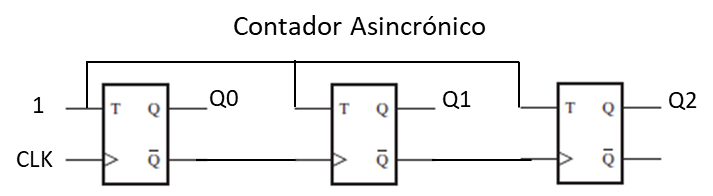
\includegraphics{../7-Async-Sync-Counter/contador asinc.png}
\end{center}

\subsection{Análisis de Ambos Circuitos}

Para poder analizar ambos circuitos, se implementó el circuito en una placa impresa (PCB) y se hizo uso de leds para hacer el circutio más interactivo.
A continuación se muestra el circuito en físico:

\begin{center}
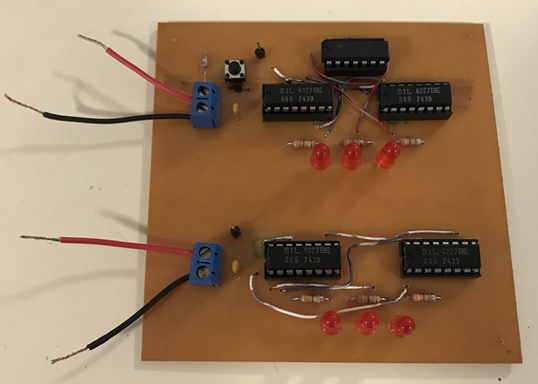
\includegraphics{../7-Async-Sync-Counter/pcb.png}
\end{center}

Luego se procedió a medir utilizando el osciloscopio la entrada y las salidas de cada estado. Y se obtuvo lo siguiente para el contador sincrónico:

